%Minimierung leer Thread
\subsection{Minimierung leer laufende Thread}

Im Cuda, bearbeitet jeder Multiprozessor gleichzeitig ein Warp von 32 Threads \cite{cudapg}, die alle zu denselben Blöcken gehören. d.h. Für sehr dumm besetzt Matrix, wie in sparse Matrixmultiplikation, sind viele Threads in Leerlauf. Um die Anzahl der in Leer laufende Thread zu minimieren, werden mehre Zeile in einem Block bearbeitet. Dazu verwendet man 2 dimensionierte Blocksizes. Die Dimension X wird hier für Elementemultiplikationen innerhalb jeweiliger Vektormultiplikationen definiert. Die Dimension Y besorgen Unterschiedlich Vektormultiplikationen innerhalb eines Blockes. Ein optimiertes Beispiel ist sparser Matrizemultiplikation, deren Implementierung ähnlich obiger Darstellung ist. Wie bestimmt man die genaue Größe für beide Dimensionen?  Man kann für speziale Anwendungen durch Folgende Versuche die beide dimensionierte Größe auswahlen. Fig[] zeigt die Laufzeit der Multiplikation Ein-Diagonalematrize mal Vektor mit unterschiedliche Blocksize. Es ist offenbar, dass für 1-Diagonalmatize das optimale Blocksize 16x1 oder 32x1 beträgt. 1-Diagonalmatize ist nicht einzige dümbesetzte Matrize in unserer Anwendung. Dickere Sparsermatrizen entstehen auch häufig. Fig[] ist die Messung für 32-Diagonalmatize. Man findet 16x16 eine schlauere Auswahl.


\begin{figure}[htbp]
%\centering

%\begin{minipage}[t]{0.3\textwidth}
%	\centering
	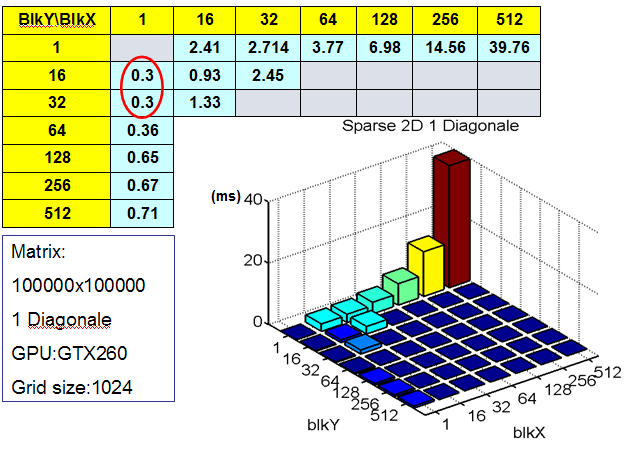
\includegraphics[width=1.7in]{../xby/pic//einDiagonal}
	\caption{Multipliktion Ein-Diagonalematrize mal Vektor. BlockY: Anzahl der Y-Dimension von Block; BlockX: Anzahl der X-Dimension von Block}
%\end{minipage}
%\begin{minipage}[t]{0.3\textwidth}
%	\centering
	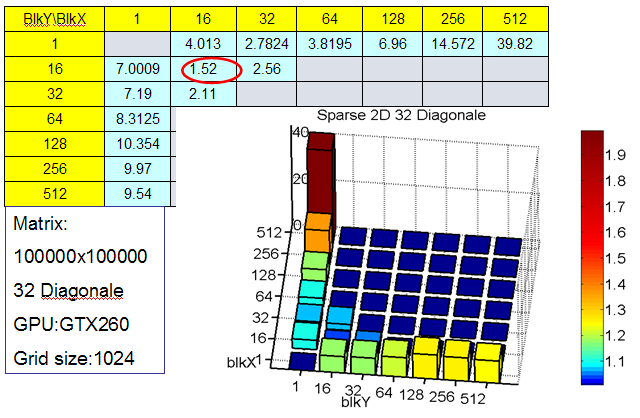
\includegraphics[width=1.7in]{../xby/pic//moreDiagonal}
	\caption{Multipliktion 32-Diagonalematrize mal Vektor. BlockY: Anzahl der Y-Dimension von Block; BlockX: Anzahl der X-Dimension von Block.}
%\end{minipage}
\end{figure}